\chapter{Graph Exploration and Structural Insights}
\label{chap:graph_exploration}

\section{Why Explore the Graph Before Prediction?}

It is tempting to treat the graph built in Chapter~\ref{chap:kg} as a
black box that is fed into a GNN and evaluated by a single F1 number.
That view is wrong for two reasons.

First, \emph{the graph is the dataset}. In a flat-text pipeline the
dataset is a set of labelled documents; here the dataset is a typed,
relational object with cross-domain structure, and any claim a later
chapter makes about the model's behaviour presupposes a concrete
understanding of that structure. Whether the model's accuracy is
driven by genuine cross-case reasoning or by a few dominant hub
statutes, whether the five legal domains are actually five or mostly
one, whether the per-case subgraph has the connectivity a
message-passing layer needs -- none of these questions can be answered
by looking at prediction results alone.

Second, \emph{leakage-safety claims are structural claims}. The
leakage prevention strategy in
Section~\ref{sec:leakage_prevention} is only as convincing as the
structural evidence that the remaining graph is still dense enough to
support learning. If removing RPC annotations, decision fields, and
identity-proxy shortcuts left behind a near-disconnected graph, the
downstream accuracy would be either implausibly high (still leaking)
or implausibly low (now uninformative). The exploration stage is
where we verify that neither is the case.

This chapter therefore treats the graph as an object of study in its
own right. Section~\ref{sec:graph_stats} summarises the overall
structure; Section~\ref{sec:perdomain} breaks it down per legal
domain; Section~\ref{sec:key_insights} distils the conclusions that
feed forward into Chapter~\ref{chap:results}.

\section{Graph Statistics and Structural Analysis}
\label{sec:graph_stats}

\subsection{Overall Graph Statistics}

The final reasoning-focused graph, assembled across all five legal
domain buckets, contains \textbf{880{,}176 nodes} and
\textbf{1{,}977{,}295 edges}. The average node degree is
\textbf{4.49}; the maximum degree is \textbf{29{,}602}, attained by
the \textsc{IPC} statute node.

At the per-bucket level (before cross-bucket sharing is expanded into
the unified view the GNN trains on), the five buckets have broadly
comparable case counts but markedly different internal densities:

\begin{table}[H]
  \centering
  \small
  \begin{adjustbox}{max width=\textwidth}
  \begin{tabular}{lrrr}
    \toprule
    Bucket & Cases (files) & Nodes & Edges \\
    \midrule
    Family \& Matrimonial & 15{,}307 & 97{,}150 & 3{,}660{,}068 \\
    Financial Fraud & 14{,}616 & 113{,}240 & 7{,}869{,}952 \\
    Land \& Property & 14{,}052 & 126{,}962 & 9{,}210{,}612 \\
    Motor Accidents & 15{,}237 & 125{,}234 & 7{,}165{,}461 \\
    Sexual Offences & 14{,}597 & 106{,}662 & 7{,}123{,}225 \\
    \midrule
    \textbf{Cross-bucket unified} & \textbf{73{,}809} & \textbf{485{,}540}
      & \textbf{27{,}243{,}141} \\
    \bottomrule
  \end{tabular}
  \end{adjustbox}
  \caption{Per-bucket and cross-bucket graph statistics. The
  cross-bucket graph is denser than the sum of the per-bucket graphs
  because shared \textsc{Statute}, \textsc{Provision}, and
  \textsc{Precedent} nodes acquire edges from every bucket that cites
  them.}
  \label{tab:graph_stats}
\end{table}

Family-matrimonial is the sparsest bucket by edges-per-case
(\(\approx 239\)), and land-property is the densest (\(\approx 655\));
the difference is driven mostly by the number of distinct provisions
and precedents cited per case in each domain.

\subsection{Node Type Distribution}

The node-type breakdown of the unified graph is strongly skewed
towards \textbf{parties and precedents}:

\begin{table}[H]
  \centering
  \small
  \begin{adjustbox}{max width=\textwidth}
  \begin{tabular}{lrr}
    \toprule
    Node type & Count & Share \\
    \midrule
    \textsc{Case} & 72{,}735 & 8.3\% \\
    \textsc{Precedent} & 255{,}148 & 29.0\% \\
    \textsc{Respondent} & 192{,}147 & 21.8\% \\
    \textsc{Petitioner} & 171{,}084 & 19.4\% \\
    \textsc{Lawyer} & 73{,}645 & 8.4\% \\
    \textsc{Provision} & 43{,}504 & 4.9\% \\
    \textsc{Court} & 38{,}799 & 4.4\% \\
    \textsc{Statute} & 21{,}754 & 2.5\% \\
    \textsc{Judge} & 11{,}360 & 1.3\% \\
    \bottomrule
  \end{tabular}
  \end{adjustbox}
  \caption{Distribution of the 880{,}176 nodes by type in the unified
  reasoning-focused graph.}
  \label{tab:node_type_dist}
\end{table}

% A per-bucket breakdown of these counts into \emph{shared} versus
% \emph{local} nodes is given in Appendix~\ref{app:shared_vs_local}.

\subsection{Degree Distribution and Hub Entities}

The graph is strongly hub-dominated. The top-12 nodes by degree are
all statutes, provisions, or courts -- exactly the node types the
schema shares across cases:

\begin{table}[H]
  \centering
  \small
  \begin{adjustbox}{max width=\textwidth}
  \begin{tabular}{llrr}
    \toprule
    Node & Type & Degree & Buckets bridged \\
    \midrule
    IPC & Statute & 29{,}602 & 5 \\
    CR.P.C. & Statute & 18{,}704 & 5 \\
    Supreme Court & Court & 17{,}294 & 5 \\
    Apex Court & Court & 14{,}242 & 5 \\
    Indian Penal Code & Statute & 12{,}009 & 5 \\
    High Court of Judicature at Allahabad & Court & 8{,}833 & 5 \\
    Section 482 & Provision & 8{,}732 & 5 \\
    Section 506 & Provision & 8{,}258 & 5 \\
    I.P.C. & Statute & 7{,}051 & 5 \\
    Section 420 & Provision & 6{,}285 & 5 \\
    Section 323 & Provision & 6{,}002 & 5 \\
    Constitution of India & Statute & 5{,}950 & 5 \\
    \bottomrule
  \end{tabular}
  \end{adjustbox}
  \caption{Top hub entities by degree, with the number of buckets they
  bridge. Every one of the top 12 hubs appears in all five legal
  domains.}
  \label{tab:top_hubs}
\end{table}

That every one of the top hubs bridges all five buckets is not an
accident: these are the statutes and courts every Indian criminal and
civil proceeding touches, and they are where cross-case message
passing actually happens.

% The full degree distribution (a complementary cumulative plot on
% log-log axes, confirming a heavy-tailed, scale-free-like shape) is in
% Appendix~\ref{app:degree_ccdf}.
The degree distribution is heavy-tailed and scale-free-like, so
cross-case reasoning capacity is structurally concentrated in a
handful of statute and court nodes; the connectivity score in
Section~\ref{sec:connectivity} quantifies how well each individual
case is wired into that hub layer.

\subsection{Cross-Domain Bridge Analysis}

The buckets are not isolated. Table~\ref{tab:top_hubs} already shows
that the top hubs are bridges by construction; the full bridge
analysis confirms that the connective tissue between domains is
dominated by the general criminal-procedure and penal-code statutes,
with domain-specific bridges layered on top:

\begin{itemize}
  \item \textsc{IPC}, \textsc{CR.P.C.}, \textsc{Indian Penal Code},
    \textsc{Constitution of India}, and \textsc{Supreme Court} /
    \textsc{Apex Court} appear in all five buckets and together account
    for the majority of cross-bucket edges.
  \item Domain-specific statutes bridge fewer buckets but at higher
    within-bucket intensity: \textsc{POCSO Act} appears in four
    buckets but is heavily concentrated in sexual-offences;
    \textsc{Motor Vehicles Act, 1988} appears in all five but is
    concentrated in motor-accidents; \textsc{Land Acquisition Act,
    1894} is concentrated in land-property.
  \item Provisions like Section~482, 506, 420, and 323 are multi-bucket
    because they sit in the CrPC and IPC, which are themselves
    multi-domain.
\end{itemize}

% A combined ranking of degree and bridging is plotted in
% Appendix~\ref{app:top_hubs_bridging}.

\subsection{Cross-Bucket Entity Sharing Matrix}

Knowing which individual nodes are hubs is useful; knowing how many entities
are shared \emph{between each pair of domains} is a different and complementary
question. If two domains share very few entities, cross-domain transfer between
them is structurally impossible, there are no shared nodes for message passing
to flow through. If two domains share nearly all entities, they are functionally
the same graph and a separate bucket structure adds no value. The cross-bucket
sharing matrix in Figure~\ref{fig:cross_bucket_sharing_matrix} quantifies this
pairwise sharing at the canonicalised entity level across the full graph.

\begin{figure}[H]
  \centering
  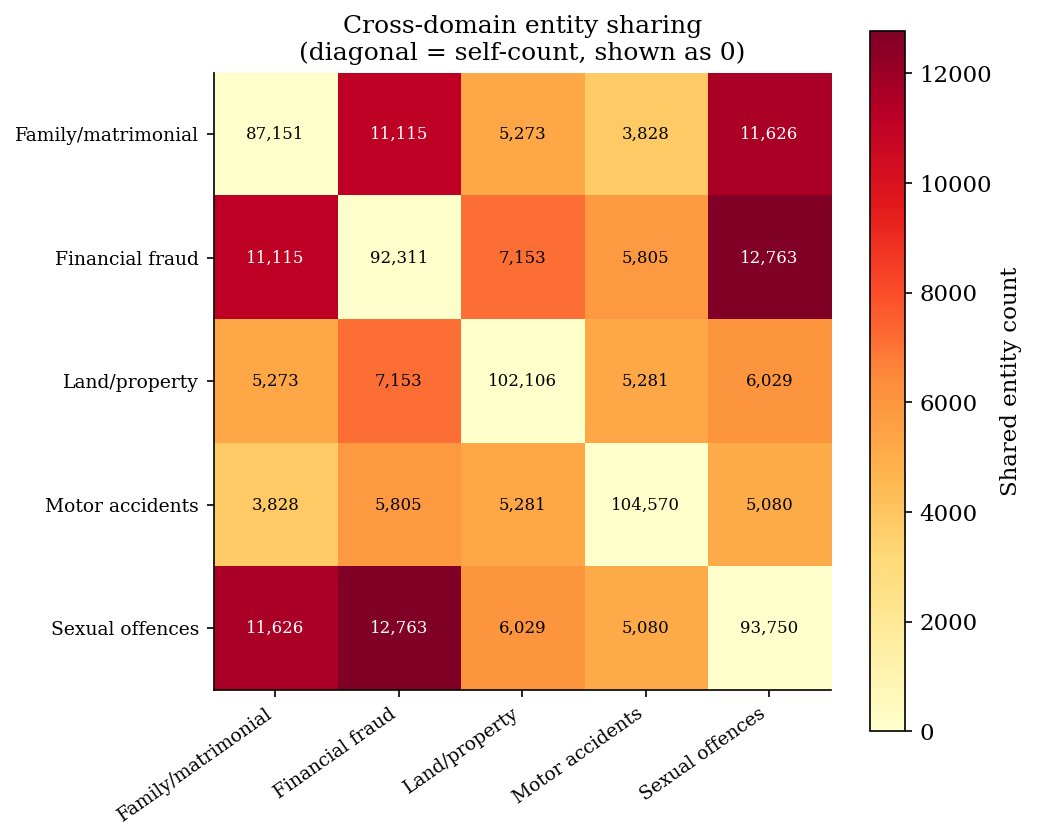
\includegraphics[width=0.9\textwidth]{figures/20_cross_bucket_sharing_matrix.png}
  \caption{Cross-bucket entity sharing matrix for the full graph. Each cell
  shows the number of canonicalised entities shared between two legal domain
  buckets. Darker values indicate more sharing. The three IPC/CrPC-driven
  buckets, family-matrimonial, financial-fraud, and sexual-offences, share
  heavily with each other; land-property is more weakly connected to the rest
  via its distinct statutory backbone.}
  \label{fig:cross_bucket_sharing_matrix}
\end{figure}

Three patterns are visible in the matrix:

\begin{enumerate}
  \item Strong pairwise sharing among \emph{Family \& Matrimonial},
    \emph{Financial Fraud}, and \emph{Sexual Offences}, all three are
    IPC/CrPC-driven and share the same high-degree statute and provision nodes.
  \item Moderate sharing between those three and \emph{Motor Accidents},
    mediated by the general procedural statutes and by the Supreme Court and High
    Court nodes that every appellate domain shares.
  \item Comparatively weaker sharing with \emph{Land \& Property}, which is
    anchored by its own statutory backbone (Land Acquisition Act~1894,
    Constitution of India) and consequently has fewer canonical entities in
    common with the criminal-procedure-dominated domains.
\end{enumerate}

This pattern is exactly what a cross-domain transfer claim needs to be credible.
The domains are related enough that a shared graph representation should carry
useful signal across all five buckets; they are different enough that each bucket
retains its own statutory fingerprint and that a single-domain classifier should
not trivially dominate a cross-domain one. The moderate but not extreme sharing
level motivates the design choice of a unified cross-bucket graph rather than
five separate per-domain graphs: there is sufficient shared structure to benefit
from joint training, but sufficient domain separation to make that benefit
non-trivial.

\subsection{Connectivity Score Distribution}
\label{sec:connectivity}

The hub analysis above characterises individual nodes; a complementary
question is how well each \emph{case} as a whole is wired into the
shared-entity layer. A bucket-normalised \textbf{connectivity score}
captures this for every case: cases that cite many hub statutes and
widely-cited precedents score high; cases that sit primarily on rare
authorities score low.
% The per-bucket distribution is plotted in
% Appendix~\ref{app:connectivity_violin}.

\section{Per-Domain Corpus Analysis}
\label{sec:perdomain}

The structural view above aggregates across buckets; the per-domain
view is where the legal character of each bucket shows up.

\subsection{Case Length and Sentence Distributions}

Case length varies substantially across buckets and directly drives
the \texttt{bge-m3} chunking strategy of
Section~\ref{sec:text_features}.
% The full per-bucket sentence-count
% distribution is in Appendix~\ref{app:sentence_count_dist}.

\subsection{Entity Richness Per Domain}

Entity richness, the number of unique canonicalised entities per
case, and mean case degree are both per-bucket structural
properties of the graph.%; the full bucket-level comparison is in
% Appendix~\ref{app:richness_and_degree}.

The PageRank ranking within each bucket makes the domain fingerprint concrete:

\begin{itemize}
  \item \textbf{Family \& Matrimonial}: IPC, CrPC, Sections~498A, 482.
  \item \textbf{Financial Fraud}: IPC, CrPC, Sections~420, 468, 471.
  \item \textbf{Land \& Property}: Supreme Court, Land Acquisition
    Act~1894, Constitution of India.
  \item \textbf{Motor Accidents}: Motor Vehicles Act~1988, Supreme Court,
    Apex Court, Section~166.
  \item \textbf{Sexual Offences}: IPC, CrPC, POCSO Act, Section~506.
\end{itemize}

The top-5 per bucket is a near-perfect fingerprint of the underlying
legal domain, which is a reassuring sanity check: the canonicalisation
and the NER are recovering legally meaningful primary citations, not
surface noise.

The ranked lists tell us \emph{which} entities are important, and
two structural patterns feed forward into the prediction chapter:
domains with spread, multi-centred geometry (land-property,
financial-fraud) carry more diversity for multi-hop message passing
to exploit than domains with tight, low-diversity backbones
(motor-accidents); and a three-tier bridge structure, universal
apex-court bridges, mid-tier IPC/CrPC bridges spanning the
criminal-procedure domains, and narrow domain-exclusive authorities
, gives the heterogeneous graph enough shared structure for
cross-domain representation learning while preserving per-domain
fingerprints.
% The ranked lists tell us \emph{which} entities are important; the
% within-bucket entity co-occurrence networks
% (Appendix~\ref{app:within_bucket_network_fingerprints}) and the
% cross-domain top-10 fingerprint
% (Appendix~\ref{app:cross_domain_network_fingerprint}) tell us
% \emph{how} they are organised. Two structural patterns from those
% appendix views feed forward into the prediction chapter: ...

\subsection{Rhetorical Role Composition Per Domain}

The rhetorical-role composition of the corpus is what tells us whether
the leakage gate from Chapter~\ref{chap:pipeline} actually fired. The
two decisive labels, \textsc{RPC} (the operative paragraph) and
\textsc{RLC} (the lower-court ruling), with \textsc{Analysis} and the
\textsc{Ratio} / \textsc{Precedent-relied} class also carrying outcome
signal, have to be absent from every bucket once cleaning is applied.
Figure~\ref{fig:rr_breakdown} shows the per-bucket role distribution
side-by-side, before filtering on the left and after filtering on the
right.

\begin{figure}[H]
  \centering
  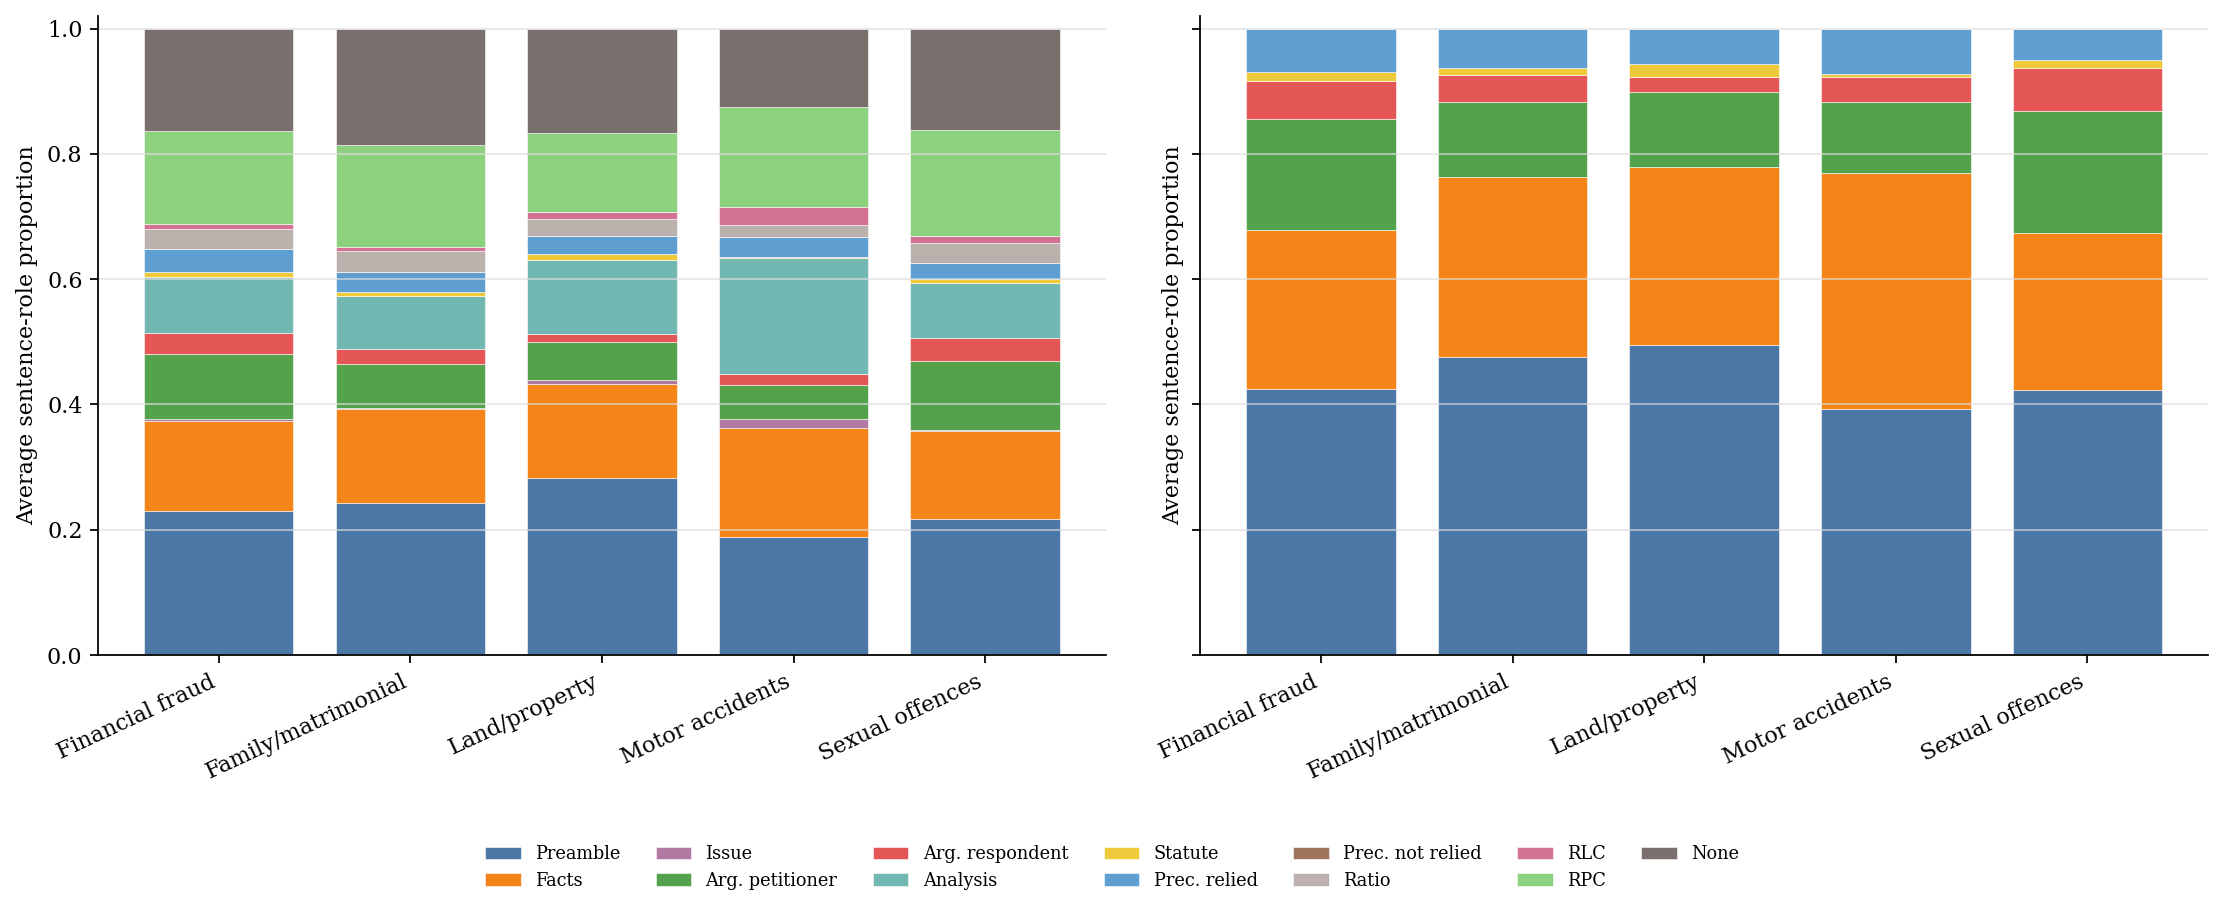
\includegraphics[width=\textwidth]{figures/new_figures/image.png}
  \caption{Rhetorical role composition per bucket before (left) and
  after (right) leakage-safe filtering. The pre-filter view contains
  the full taxonomy, including \textsc{RPC}, \textsc{RLC},
  \textsc{Ratio}, \textsc{Analysis}, and the precedent-relied / not-%
  relied roles. The post-filter view retains only \textsc{Preamble},
  \textsc{Facts}, petitioner and respondent arguments, and the
  precedent-relied trace.}
  \label{fig:rr_breakdown}
\end{figure}

The contrast between the two panels is the structural confirmation
that the leakage filter is doing what it is supposed to. On the left,
every bucket carries a visible \textsc{RPC}, \textsc{RLC}, and
\textsc{Analysis} share, together with a \textsc{None}-class residual.
On the right, those decisive bands are gone in every bucket, the
post-filter composition collapses onto \textsc{Preamble}, \textsc{Facts},
and the two argument streams, with only the precedent-relied trace
retained as non-decisive citation context. The remaining
\textsc{Facts} and \textsc{Arguments} mass is what the GNN actually
trains on, and its relative size still tracks case length: land-property
and financial-fraud carry the largest \textsc{Arguments} share,
motor-accidents the smallest, consistent with the sentence-count
ordering noted earlier in this chapter.

\subsection{Outcome Distribution Per Domain}

The outcome label distribution and its per-domain win/loss rates were analysed
in detail as part of the pipeline audit in
Chapter~\ref{chap:pipeline} (Figure~\ref{fig:outcome_rate}). From the
graph-exploration perspective, the relevant
structural observation is that the class imbalance is \emph{domain-dependent}:
motor-accidents is the most win-skewed, financial-fraud and sexual-offences sit
closest to balanced. This means the GNN's training signal is not uniformly
imbalanced, different domains present different prior odds, which in turn
means that per-domain calibration, rather than a single global threshold,
is the appropriate evaluation design. The cross-bucket pooled win rate of
roughly $60\%$ to $40\%$ is why Chapter~\ref{chap:results} reports macro-F1
alongside accuracy and ROC-AUC as co-primary metrics.

\section{Key Structural Insights}
\label{sec:key_insights}

Five insights carry forward into the prediction chapter:

\begin{enumerate}
  \item \textbf{The graph is hub-dominated.} A small number of
    cross-bucket statutes and courts (IPC, CrPC, Supreme Court) are
    the spine of the graph; most other entities are long-tail leaves.
    Any claim the model makes about ``cross-case reasoning'' must be
    interpretable against this topology.
  \item \textbf{Cross-domain sharing is real but uneven.} The four
    IPC/CrPC-driven buckets share heavily with each other; land-property
    partially detaches via its own statutory backbone. A cross-domain
    model should outperform a naive concatenation only if it can
    actually exploit the shared spine.
  \item \textbf{Identity-proxy leakage is structural.} Judges,
    specific lawyers, and specific courts have bridge and betweenness
    scores high enough to make \emph{sharing} them across cases
    unsafe; the decision to hold them local is vindicated by the
    bridge analysis.
  \item \textbf{Connectivity score predicts modelling difficulty.}
    Low-connectivity cases have, by construction, fewer shared-entity
    neighbours to aggregate from; the per-domain accuracy pattern in
    Chapter~\ref{chap:results} is consistent with connectivity being a
    first-order driver of case-level difficulty.
  \item \textbf{The per-domain fingerprints are legally coherent.}
    Each bucket's top-PageRank entities are exactly what a lawyer
    would expect; this is the single strongest evidence that the
    pipeline's NER, canonicalisation, and rhetorical-role filtering
    together produce a legally faithful, not merely statistically
    clean, corpus.
\end{enumerate}
